
%     * without a RnD budget, little innovation comes out of Tanzania. However, the country still greatly benefits from new innovations from other countries.

%     * The average tanzanian walks 6km daily to get water. On their daily walk, are they going to be thinking about their CO2 emissions and impact on the environment? Probably not. 

%     * Where the grid is limited or non-existent, portable renewable energy systems are needed. 

%     The majority of energy in Tanzania is sourced from Bio fuel. While this is renewable, it is not sustainable.

%     Hydro Power is most prevalent source of electricity

%     Solar Power becoming prevalent in Tanzania. on the equator where the sun is always shining. 

%     * Where the energy comes from and the impact -- biomass-> burning of palm oils and wood. makes for 90 percent of energy consumption. renewable but not sustainable. bad for the environment, however not of concern to Tanzania.
% 1/3rd of electricity is generated by hydroelectric power plants. potential for much more. 


% The majority of Tanzania's energy needs are met with renewable energy, resulting in a very low, CO2 intensity of energy mix of 11.9t/Tj. 90\% of energy consumption comes from the burning of biomass. About 1/3rd of electricity is generated by hydroelectric power plants. 

% While the tanzania does not have a rnd budget, it still greatly benefits from new innovations from other countries. 





% Tanzania is beginning to adopt solar power as a means to modernism the country. Low powered electronics are becoming more common, and the country is beginning to adopt solar powered street lights.


% * renewable energy in tanzania. --> break down of RE energy profile

% * why renewable energy is important. -> sustainable energy, minimal running cost, no need to import fuel. 

% * how renewable energy innovations in tanzania. -> introduction of electronics. low power electionics are cheap luxuries. with lack of infrastructure


% * majority of energy consumption comes from residential stuff. 


% * why renewable energy is relevant in a country like Tanzania



Around 90 \% of the energy consumption comes from burning biomass, a renewable energy source; however, it is not sustainable. Burning biomass is terrible for the environment; however, this is generally not of concern to Tanzania due to its economic status. 



    \begin{figure}
        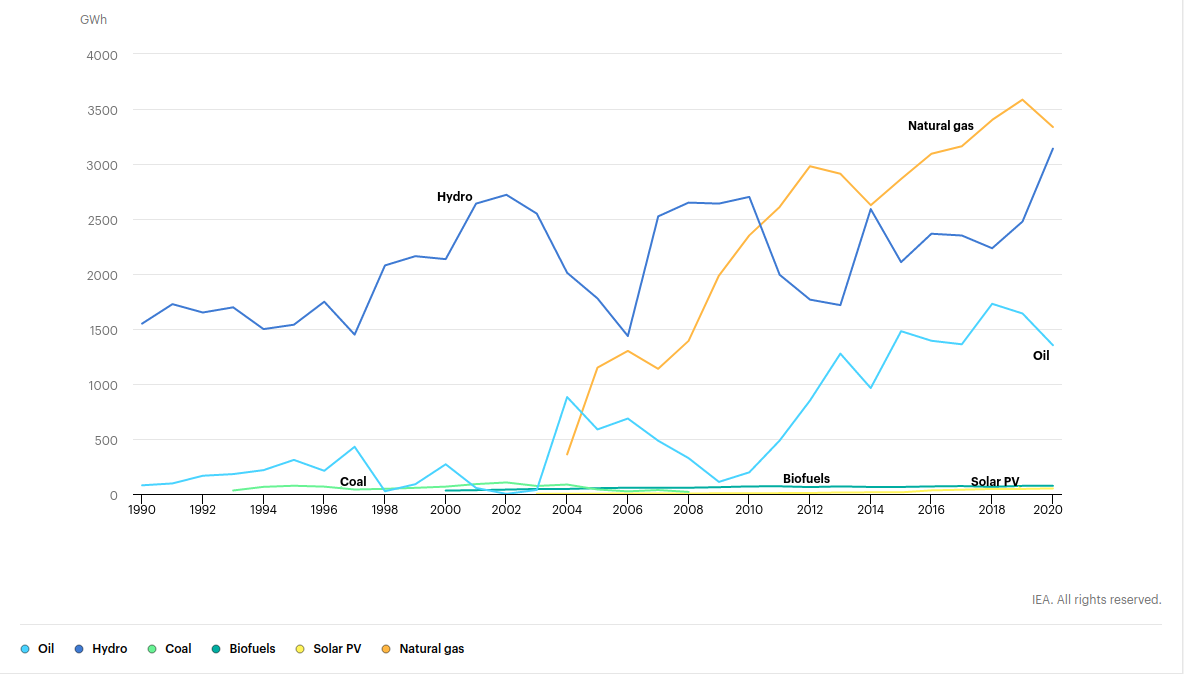
\includegraphics[width=0.8\textwidth]{IMG/Screenshot from 2023-03-15 12-36-31.png}
        \caption{Electricity generation by source in Tanzania \cite{iea}}
        \end{figure}\label{fig:4_Review_1}
    
